\newpage
%Nicht anfassen, so ist der Dokumentenaufbau
% \addtocontents{toc}{\protect\setcounter{tocdepth}{0}}
% \renewcommand{\appendixtocname}{Anhang}
% \addappheadtotoc % Überschrift 'Anhang' in TOC
\renewcommand{\appendixpagename}{Appendix}
\appendix
\appendixpage
\appendixtitleoff
% \section*{Appendix}
% \appendix
\addcontentsline{toc}{section}{Appendix}
\setlength{\footskip}{35pt}

\renewcommand{\figurename}{Appendix Figure}
\renewcommand{\tablename}{Appendix Table}
\setcounter{figure}{0} 
\setcounter{table}{0}
% \crefalias{figure}{appfig}
% \crefalias{table}{apptab}
% \crefalias{section}{appsec}

% \todo[inline]{align numerical cols to the right}

% ll FBA variants
\begin{table}[!ht]
    \small
    \centering
    \addtolength{\leftskip} {-2cm}
    \addtolength{\rightskip}{-2cm}
    \begin{tabular}{@{\extracolsep{4pt}}llrrlrr@{}}
    \hline
        \multicolumn{1}{c}{} & \multicolumn{3}{c}{\textbf{ll-FBA (big-M)}} & \multicolumn{3}{c}{\textbf{ll-FBA (nullspace)}}\\ \cline{2-4} \cline{5-7} 
        \textbf{organism} & \textbf{termination} & \textbf{time} & \thead{objective \\value} & \textbf{termination} & \textbf{time} & \thead{objective \\value} \\ \hline
        e\_coli\_core & OPTIMAL & 0 & 0.874 & OPTIMAL & 0 & 0.874 \\
        iAB\_RBC\_283 & OPTIMAL & 0 & 2.936 & OPTIMAL & 2 & 2.936 \\
        iIS312\_Amastigote & OPTIMAL & 0 & 25.339 & OPTIMAL & 0 & 25.339 \\
        iAF692 & OPTIMAL & 0 & 0.0 & TIME\_LIMIT & 1800 & 0.026 \\
        iSB619 & OPTIMAL & 0 & 0.0 & TIME\_LIMIT & 1800 & 0.027 \\
        iNF517 & OPTIMAL & 9 & 0.043 & OPTIMAL & 39 & 0.043 \\
        iHN637 & OPTIMAL & 4 & 0.224 & OPTIMAL & 5 & 0.224 \\
        iJB785 & OPTIMAL & 15 & 0.054 & OPTIMAL & 25 & 0.0 \\
        iNJ661 & TIME\_LIMIT & 1800 & 0.014 & OPTIMAL & 227 & 0.053 \\ 
        % iSynCJ816 & OPTIMAL & 1 & 0.0 & INFEASIBLE & 34 & - \\
        iJN746 & OPTIMAL & 332 & 1.4 & TIME\_LIMIT & 1800 & - \\
        iJR904 & OPTIMAL & 9 & 0.0 & OPTIMAL & 163 & 0.922 \\
        iEK1008 & OPTIMAL & 473 & 0.0 & OPTIMAL & 503 & 0.058 \\
        iCN900 & OPTIMAL & 0 & 0.0 & OPTIMAL & 27 & 0.0 \\
        iYO844 & TIME\_LIMIT & 1800 & 0.115 & TIME\_LIMIT & 1800 & 0.0 \\
        iND750 & OPTIMAL & 8 & 0.0 & OPTIMAL & 151 & 0.0 \\
        iMM904 & OPTIMAL & 650 & 0.277 & TIME\_LIMIT & 1800 & 0.0 \\
        iRC1080 & OPTIMAL & 373 & 0.0 & TIME\_LIMIT & 1800 & - \\
        iAF1260 & TIME\_LIMIT & 1800 & 0.0 & TIME\_LIMIT & 1800 & 0.0 \\
        iSDY\_1059 & OPTIMAL & 1457 & 0.938 & TIME\_LIMIT & 1800 & 0.0 \\
        STM\_v1\_0 & TIME\_LIMIT & 1800 & 0.0 & TIME\_LIMIT & 1800 & 0.0 \\
        iJO1366 & TIME\_LIMIT & 1800 & 0.0 & TIME\_LIMIT & 1800 & 0.0 \\
        iSbBS512\_1146 & TIME\_LIMIT & 1800 & 0.0 & TIME\_LIMIT & 1800 & 0.0 \\
        iS\_1188 & TIME\_LIMIT & 1800 & 0.832 & TIME\_LIMIT & 1800 & 0.0 \\
        iSFV\_1184 & OPTIMAL & 1710 & 0.894 & TIME\_LIMIT & 1800 & 0.0 \\
        iSF\_1195 & OPTIMAL & 1584 & 0.915 & TIME\_LIMIT & 1800 & -0.0 \\
        iSFxv\_1172 & OPTIMAL & 966 & 0.894 & TIME\_LIMIT & 1800 & 0.0 \\
        iML1515 & TIME\_LIMIT & 1800 & 0.861 & TIME\_LIMIT & 1800 & - \\
        iZ\_1308 & TIME\_LIMIT & 1800 & 0.0 & TIME\_LIMIT & 1800 & 0.0 \\
        iAPECO1\_1312 & TIME\_LIMIT & 1800 & 0.934 & TIME\_LIMIT & 1800 & 0.0 \\
        iECB\_1328 & TIME\_LIMIT & 1800 & 0.0 & TIME\_LIMIT & 1800 & 0.0 \\
        iETEC\_1333 & TIME\_LIMIT & 1800 & 0.0 & TIME\_LIMIT & 1800 & 0.0 \\
        iYS1720 & TIME\_LIMIT & 1800 & 0.0 & TIME\_LIMIT & 1800 & - \\
        iMM1415 & OPTIMAL & 1550 & 0.0 & TIME\_LIMIT & 1800 & - \\
        RECON1 & OPTIMAL & 83 & 0.0 & TIME\_LIMIT & 1800 & - \\
        iLB1027\_lipid & TIME\_LIMIT & 1800 & 0.0 & TIME\_LIMIT & 1800 & - \\
        Recon3D & TIME\_LIMIT & 1800 & - & TIME\_LIMIT & 1800 & - \\ \hline
    \end{tabular}
    \caption{\label[apptab]{tab:ll_fba_comparison} Results of using the nullspace formulation vs the reformulation.}
\end{table}
\todo[inline]{check iJB785}

\begin{table}[!ht]
    \small
    \centering
    \addtolength{\leftskip} {-2cm}
    \addtolength{\rightskip}{-2cm}
    \begin{tabular}{@{\extracolsep{4pt}}llrrlrr@{}}
    \hline
        \multicolumn{1}{c}{} & \multicolumn{3}{c}{\textbf{ll-FBA (big-M)}} & \multicolumn{3}{c}{\textbf{ll-FBA (indicator)}}\\ \cline{2-4} \cline{5-7} 
        \textbf{organism} & \textbf{termination} & \textbf{time} & \thead{objective \\value} & \textbf{termination} & \textbf{time} & \thead{objective \\value} \\ \hline
        e\_coli\_core & OPTIMAL & 0 & 0.874 & OPTIMAL & 0 & 0.874 \\ 
        iAB\_RBC\_283 & OPTIMAL & 0 & 2.936 & OPTIMAL & 1 & 2.936 \\ 
        iIS312\_Amastigote & OPTIMAL & 0 & 25.339 & OPTIMAL & 1 & 25.339 \\ 
        iAF692 & OPTIMAL & 0 & 0.0 & TIME\_LIMIT & 1800 & - \\ 
        iSB619 & OPTIMAL & 0 & 0.0 & INFEASIBLE & 2 & - \\ 
        iNF517 & OPTIMAL & 9 & 0.043 & OPTIMAL & 19 & 0.043 \\ 
        iHN637 & OPTIMAL & 4 & 0.224 & OPTIMAL & 64 & 0.224 \\ 
        iJB785 & OPTIMAL & 15 & 0.054 & OPTIMAL & 429 & 0.054 \\ 
        iNJ661 & TIME\_LIMIT & 1800 & 0.014 & TIME\_LIMIT & 1800 & 0.0 \\ 
        % iSynCJ816 & OPTIMAL & 1 & 0.0 & INFEASIBLE & 0 & - \\ 
        iJN746 & OPTIMAL & 332 & 1.4 & OPTIMAL & 10 & 1.4 \\ 
        iJR904 & OPTIMAL & 9 & 0.0 & TIME\_LIMIT & 1800 & 0.0 \\ 
        iEK1008 & OPTIMAL & 473 & 0.0 & TIME\_LIMIT & 1800 & 0.0 \\ 
        iCN900 & OPTIMAL & 0 & 0.0 & OPTIMAL & 4 & 0.0 \\ 
        iYO844 & TIME\_LIMIT & 1800 & 0.115 & TIME\_LIMIT & 1800 & 0.118 \\ 
        iND750 & OPTIMAL & 8 & 0.0 & TIME\_LIMIT & 1800 & 0.0 \\ 
        iMM904 & OPTIMAL & 650 & 0.277 & TIME\_LIMIT & 1800 & - \\ 
        iRC1080 & OPTIMAL & 373 & 0.0 & TIME\_LIMIT & 1800 & - \\ 
        iAF1260 & TIME\_LIMIT & 1800 & 0.0 & TIME\_LIMIT & 1800 & - \\ 
        iSDY\_1059 & OPTIMAL & 1457 & 0.938 & TIME\_LIMIT & 1800 & - \\ 
        STM\_v1\_0 & TIME\_LIMIT & 1800 & 0.0 & TIME\_LIMIT & 1800 & - \\ 
        iJO1366 & TIME\_LIMIT & 1800 & 0.0 & TIME\_LIMIT & 1800 & - \\ 
        iSbBS512\_1146 & TIME\_LIMIT & 1800 & 0.0 & TIME\_LIMIT & 1800 & - \\ 
        iS\_1188 & TIME\_LIMIT & 1800 & 0.832 & TIME\_LIMIT & 1800 & 0.0 \\ 
        iSFV\_1184 & OPTIMAL & 1710 & 0.894 & TIME\_LIMIT & 1800 & - \\ 
        iSF\_1195 & OPTIMAL & 1584 & 0.915 & TIME\_LIMIT & 1800 & - \\ 
        iSFxv\_1172 & OPTIMAL & 966 & 0.894 & TIME\_LIMIT & 1800 & - \\ 
        iML1515 & TIME\_LIMIT & 1800 & 0.861 & TIME\_LIMIT & 1800 & - \\ 
        iZ\_1308 & TIME\_LIMIT & 1800 & 0.0 & TIME\_LIMIT & 1800 & - \\ 
        iAPECO1\_1312 & TIME\_LIMIT & 1800 & 0.934 & TIME\_LIMIT & 1800 & 0.0 \\ 
        iECB\_1328 & TIME\_LIMIT & 1800 & 0.0 & TIME\_LIMIT & 1800 & - \\ 
        iETEC\_1333 & TIME\_LIMIT & 1800 & 0.0 & TIME\_LIMIT & 1800 & - \\ 
        iYS1720 & TIME\_LIMIT & 1800 & 0.0 & TIME\_LIMIT & 1800 & - \\ 
        iMM1415 & OPTIMAL & 1550 & 0.0 & OPTIMAL & 71 & 0.0 \\ 
        RECON1 & OPTIMAL & 83 & 0.0 & OPTIMAL & 76 & 0.0 \\ 
        iLB1027\_lipid & TIME\_LIMIT & 1800 & 0.0 & TIME\_LIMIT & 1800 & - \\ 
        Recon3D & TIME\_LIMIT & 1800 & - & TIME\_LIMIT & 1800 & - \\ \hline
    \end{tabular}
    \caption{\label[apptab]{tab:ll_fba_indicator} Results of using the big-M formulation vs the indicator formulation.}
\end{table}

% \begin{table}[!ht]
%     \small
%     \centering
%     \begin{tabular}{@{\extracolsep{4pt}}lllllll@{}}
%     \hline
%         \multicolumn{1}{c}{} & \multicolumn{3}{c}{\textbf{ll-FBA (big-M)}} & \multicolumn{3}{c}{\textbf{ll-FBA (indicator)}}\\ \cline{2-4} \cline{5-7} 
%         \textbf{organism} & \textbf{termination} & \textbf{time} & \thead{objective \\value} & \textbf{termination} & \textbf{time} & \thead{objective \\value} \\ \hline
%         e\_coli\_core & OPTIMAL & 0 & 0.874 & OPTIMAL & 1 & -0.0 \\ \hline
%         iAB\_RBC\_283 & OPTIMAL & 0 & 2.936 & TIME\_LIMIT & 1800 & 2.936 \\ \hline
%         iIS312\_Amastigote & OPTIMAL & 0 & 25.339 & INFEASIBLE & 1 & - \\ \hline
%         iAF692 & OPTIMAL & 0 & 0.0 & TIME\_LIMIT & 1800 & - \\ \hline
%         iSB619 & OPTIMAL & 0 & 0.0 & INFEASIBLE & 3 & - \\ \hline
%         iNF517 & OPTIMAL & 9 & 0.043 & INFEASIBLE & 7 & - \\ \hline
%         iHN637 & OPTIMAL & 4 & 0.224 & INFEASIBLE & 1 & - \\ \hline
%         iJB785 & OPTIMAL & 15 & 0.054 & OPTIMAL & 764 & 0.054 \\ \hline
%         iNJ661 & TIME\_LIMIT & 1800 & 0.014 & INFEASIBLE & 3 & - \\ \hline
%         iSynCJ816 & OPTIMAL & 1 & 0.0 & INFEASIBLE & 0 & - \\ \hline
%         iJN746 & OPTIMAL & 332 & 1.4 & TIME\_LIMIT & 1800 & - \\ \hline
%         iJR904 & OPTIMAL & 9 & 0.0 & TIME\_LIMIT & 1800 & - \\ \hline
%         iEK1008 & OPTIMAL & 473 & 0.0 & TIME\_LIMIT & 1800 & - \\ \hline
%         iCN900 & OPTIMAL & 0 & 0.0 & INFEASIBLE & 8 & - \\ \hline
%         iYO844 & TIME\_LIMIT & 1800 & 0.115 & TIME\_LIMIT & 1800 & - \\ \hline
%         iND750 & OPTIMAL & 8 & 0.0 & INFEASIBLE & 61 & - \\ \hline
%         iMM904 & OPTIMAL & 650 & 0.277 & INFEASIBLE & 4 & - \\ \hline
%         iRC1080 & OPTIMAL & 373 & 0.0 & TIME\_LIMIT & 1800 & - \\ \hline
%         iAF1260 & TIME\_LIMIT & 1800 & 0.0 & TIME\_LIMIT & 1800 & - \\ \hline
%         iSDY\_1059 & OPTIMAL & 1457 & 0.938 & TIME\_LIMIT & 1800 & - \\ \hline
%         STM\_v1\_0 & TIME\_LIMIT & 1800 & 0.0 & INFEASIBLE & 2 & - \\ \hline
%         iJO1366 & TIME\_LIMIT & 1800 & 0.0 & TIME\_LIMIT & 1800 & - \\ \hline
%         iSbBS512\_1146 & TIME\_LIMIT & 1800 & 0.0 & TIME\_LIMIT & 1800 & - \\ \hline
%         iS\_1188 & TIME\_LIMIT & 1800 & 0.832 & TIME\_LIMIT & 1800 & - \\ \hline
%         iSFV\_1184 & OPTIMAL & 1710 & 0.894 & TIME\_LIMIT & 1800 & - \\ \hline
%         iSF\_1195 & OPTIMAL & 1584 & 0.915 & TIME\_LIMIT & 1800 & - \\ \hline
%         iSFxv\_1172 & OPTIMAL & 966 & 0.894 & TIME\_LIMIT & 1800 & - \\ \hline
%         iML1515 & TIME\_LIMIT & 1800 & 0.861 & TIME\_LIMIT & 1800 & - \\ \hline
%         iZ\_1308 & TIME\_LIMIT & 1800 & 0.0 & TIME\_LIMIT & 1800 & - \\ \hline
%         iAPECO1\_1312 & TIME\_LIMIT & 1800 & 0.934 & TIME\_LIMIT & 1800 & - \\ \hline
%         iECB\_1328 & TIME\_LIMIT & 1800 & 0.0 & TIME\_LIMIT & 1800 & - \\ \hline
%         iETEC\_1333 & TIME\_LIMIT & 1800 & 0.0 & TIME\_LIMIT & 1800 & - \\ \hline
%         iYS1720 & TIME\_LIMIT & 1800 & 0.0 & INFEASIBLE & 6 & - \\ \hline
%         iMM1415 & OPTIMAL & 1550 & 0.0 & TIME\_LIMIT & 1800 & - \\ \hline
%         RECON1 & OPTIMAL & 83 & 0.0 & INFEASIBLE & 8 & - \\ \hline
%         iLB1027\_lipid & TIME\_LIMIT & 1800 & 0.0 & TIME\_LIMIT & 1800 & - \\ \hline
%         Recon3D & TIME\_LIMIT & 1800 & - & TIME\_LIMIT & 1800 & - \\ \hline
%     \end{tabular}
%     \caption{\label[apptab]{tab:ll_fba_indicator} Results of using the big-M formulation vs the indicator formulation.}
% \end{table}

% blocked cycles table
\begin{table}[!ht]
    \centering
    \begin{tabular}{lrr}
    \hline
        \textbf{organism} & \textbf{time (s)} & \textbf{cycles} \\ \hline
        e\_coli\_core & 0.77 & 44 \\ 
        iCN900 & 50.47 & 191 \\ 
        iAF692 & 16.74 & 179 \\ 
        iJR904 & 42.58 & 489 \\ 
        iNJ661 & 38.08 & 510 \\ 
        iEK1008 & 58.04 & 547 \\ 
        iMM904 & 94.89 & 774 \\ 
        iSFV\_1184 & 264.95 & 1100 \\ 
        iML1515 & 318.34 & 1237 \\ \hline
    \end{tabular}
    \caption{\label[apptab]{tab:cff_time} Running time and number of detected cycles by using the CycleFreeFlux algorithm.}
\end{table}

% \todo[inline]{add results for different SCIP seeds}
% \begin{table}[!ht]
%     \centering
%     \begin{tabular}{lrrrr}
%     \hline 
%         \thead{ll-FBA \\ cycles blocked} & & & & \\ \hline
%         \textbf{block limit} & 10 & 20 & 50 & 100 \\
%         \textbf{organism} & time (s) & time (s) & time (s) & time (s) \\ \hline
%         e\_coli\_core & 0 & 0 & 0 & 0 \\ 
%         iAF692 & 6 & 4 & 7 & 14 \\ 
%         iCN900 & 0 & 0 & 0 & 0 \\ 
%         iJR904 & 29 & 30 & 20 & 16 \\ 
%         iEK1008 & 411 & 101 & 70 & 82 \\
%         iMM904 & 880 & 781 & 1689 & 1800 \\ 
%         iSFV\_1184 & 1178 & 1800 & 854 & 685 \\ 
%         iML1515 & 1800 & 1800 & 1800 & 1800 \\ 
%         iNJ661 & 134 & 89 & 163 & 79 \\ \hline
%     \end{tabular}
%     \caption{\label[apptab]{tab:cff}Runtime of ll-FBA with cycles blocked. Block limit denotes the maximal number of blocked cycles. The cycles are computed by the CycleFreeFlux algorithm.}
% \end{table}

% \begin{table}[!ht]
%     \centering
%     \begin{tabular}{lrrrr}
%         \hline 
%         \thead{ll-FBA \\ shortest cycles \\ blocked} & & & & \\ \hline
%         \textbf{block limit} & 10 & 20 & 50 & 100 \\
%         \textbf{organism} & time (s) & time (s) & time (s) & time (s) \\ \hline
%         e\_coli\_core & 0 & 0 & 0 & 0 \\ 
%         iAF692 & 5 & 4 & 7 & 14 \\
%         iCN900 & 0 & 0 & 0 & 0 \\
%         iJR904 & 40 & 39 & 27 & 72 \\
%         iEK1008 & 163 & 125 & 370 & 69 \\
%         iMM904 & 656 & 1111 & 548 & 1165 \\
%         iSFV\_1184 & 1800 & 1800 & 1800 & 1565 \\
%         iML1515 & 1800 & 1800 & 1800 & 1800 \\
%         iNJ661 & 1800 & 280 & 53 & 37 \\
%     \end{tabular}
%     \caption{\label[apptab]{tab:cff_shortest_cycles}Runtime of ll-FBA with shortest cycles blocked. Block limit denotes the maximal number of blocked cycles. The cycles are computed by the CycleFreeFlux algorithm.}
% \end{table}

% \begin{table}[!ht]
%     \small
%     \centering
%     \begin{tabular}{|l|l|l|l|l|l|l|}
%     \hline
%     \multicolumn{1}{|c}{} & \multicolumn{3}{|c|}{ll-FBA} & \multicolumn{3}{c|}{ll-FBA (nullspace)}\\ \hline 
%     \textbf{organism} & \textbf{termination} & \textbf{o. v.} & \textbf{time (s)} & \textbf{termination} & \textbf{o. v.} & \textbf{time (s)} \\ \hline    
%         e\_coli\_core & OPTIMAL & 0.874 & 0 & OPTIMAL & 0.874 & 0 \\ \hline
%         iAB\_RBC\_283 & OPTIMAL & 2.936 & 0 & OPTIMAL & 2.936 & 2 \\ \hline
%         iIS312\_Amastigote & OPTIMAL & 25.339 & 0 & OPTIMAL & 25.339 & 0 \\ \hline
%         iAF692 & OPTIMAL & 0.027 & 3 & TIME\_LIMIT & 0.026 & 1800 \\ \hline
%         iSB619 & INFEASIBLE & NaN & 1 & TIME\_LIMIT & 0.027 & 1800 \\ \hline
%         iNF517 & OPTIMAL & 0.043 & 11 & OPTIMAL & 0.043 & 39 \\ \hline
%         iHN637 & OPTIMAL & 0.224 & 4 & OPTIMAL & 0.224 & 5 \\ \hline
%         iJB785 & OPTIMAL & 0.054 & 15 & OPTIMAL & 0.0 & 25 \\ \hline
%         iNJ661 & OPTIMAL & 0.053 & 181 & OPTIMAL & 0.053 & 227 \\ \hline
%         iSynCJ816 & OPTIMAL & 0.0 & 1 & INFEASIBLE & NaN & 34 \\ \hline
%         iJN746 & OPTIMAL & 1.4 & 332 & TIME\_LIMIT & NaN & 1800 \\ \hline
%         iJR904 & OPTIMAL & 0.922 & 93 & OPTIMAL & 0.922 & 163 \\ \hline
%         iEK1008 & OPTIMAL & 0.058 & 865 & OPTIMAL & 0.058 & 503 \\ \hline
%         iCN900 & OPTIMAL & 0.0 & 0 & OPTIMAL & 0.0 & 27 \\ \hline
%         iYO844 & TIME\_LIMIT & 0.115 & 1800 & TIME\_LIMIT & 0.0 & 1800 \\ \hline
%         iND750 & OPTIMAL & 0.0 & 8 & OPTIMAL & 0.0 & 151 \\ \hline
%         iMM904 & OPTIMAL & 0.288 & 1465 & TIME\_LIMIT & 0.0 & 1800 \\ \hline
%         iRC1080 & OPTIMAL & 0.0 & 373 & TIME\_LIMIT & NaN & 1800 \\ \hline
%         iAF1260 & TIME\_LIMIT & 0.69 & 1800 & TIME\_LIMIT & 0.0 & 1800 \\ \hline
%         iSDY\_1059 & TIME\_LIMIT & 0.92 & 1800 & TIME\_LIMIT & 0.0 & 1800 \\ \hline
%         STM\_v1\_0 & TIME\_LIMIT & 0.0 & 1800 & TIME\_LIMIT & 0.0 & 1800 \\ \hline
%         iJO1366 & TIME\_LIMIT & 0.939 & 1800 & TIME\_LIMIT & 0.0 & 1800 \\ \hline
%         iSbBS512\_1146 & TIME\_LIMIT & 0.0 & 1800 & TIME\_LIMIT & 0.0 & 1800 \\ \hline
%         iS\_1188 & TIME\_LIMIT & 0.73 & 1800 & TIME\_LIMIT & 0.0 & 1800 \\ \hline
%         iSFV\_1184 & OPTIMAL & 0.894 & 1241 & TIME\_LIMIT & 0.0 & 1800 \\ \hline
%         iSF\_1195 & TIME\_LIMIT & 0.915 & 1800 & TIME\_LIMIT & -0.0 & 1800 \\ \hline
%         iSFxv\_1172 & OPTIMAL & 0.894 & 966 & TIME\_LIMIT & 0.0 & 1800 \\ \hline
%         iML1515 & OPTIMAL & 0.877 & 1692 & TIME\_LIMIT & NaN & 1800 \\ \hline
%         iZ\_1308 & TIME\_LIMIT & 0.0 & 1800 & TIME\_LIMIT & 0.0 & 1800 \\ \hline
%         iAPECO1\_1312 & TIME\_LIMIT & 0.934 & 1800 & TIME\_LIMIT & 0.0 & 1800 \\ \hline
%         iECB\_1328 & TIME\_LIMIT & 0.0 & 1800 & TIME\_LIMIT & 0.0 & 1800 \\ \hline
%         iETEC\_1333 & TIME\_LIMIT & 0.0 & 1800 & TIME\_LIMIT & 0.0 & 1800 \\ \hline
%         iYS1720 & TIME\_LIMIT & 0.0 & 1800 & TIME\_LIMIT & NaN & 1800 \\ \hline
%         iMM1415 & OPTIMAL & 0.0 & 1550 & TIME\_LIMIT & NaN & 1800 \\ \hline
%         RECON1 & OPTIMAL & 0.0 & 83 & TIME\_LIMIT & NaN & 1800 \\ \hline
%         iLB1027\_lipid & TIME\_LIMIT & 0.0 & 1800 & TIME\_LIMIT & NaN & 1800 \\ \hline
%         Recon3D & TIME\_LIMIT & NaN & 1800 & TIME\_LIMIT & NaN & 1800 \\ \hline
%     \end{tabular}
%     \caption{\label{Tab:ll_fba_comparison} Results of using the nullspace formulation vs the reformulation.}
% \end{table}

% \begin{table}[!ht]
%     \small
%     \centering
%     \begin{tabular}{|l|l|l|l|l|l|l|}
%     \hline
%     \multicolumn{1}{|c}{} & \multicolumn{2}{|c|}{ll-FBA} & \multicolumn{2}{|c|}{CB (indicator)} & \multicolumn{2}{c|}{CB (big-M)}\\ \hline 
%     organism & termination & time & termination & time & termination & time \\ \hline
%         iAF692 & OPTIMAL & 3 & OPTIMAL & 16.0 & OPTIMAL & 7.0 \\ \hline
%         iSB619 & INFEASIBLE & 1 & OPTIMAL & 15.0 & OPTIMAL & 6.0 \\ \hline
%         iNF517 & OPTIMAL & 11 & OPTIMAL & 29.0 & OPTIMAL & 12.0 \\ \hline
%         iHN637 & OPTIMAL & 4 & OPTIMAL & 11.0 & OPTIMAL & 7.0 \\ \hline
%         iJB785 & OPTIMAL & 15 & OPTIMAL & 14.0 & OPTIMAL & 7.0 \\ \hline
%         iNJ661 & OPTIMAL & 181 & OPTIMAL & 61.0 & OPTIMAL & 9.0 \\ \hline
%         iSynCJ816 & OPTIMAL & 1 & ERROR & NaN & ERROR & NaN \\ \hline
%         iJN746 & OPTIMAL & 332 & OPTIMAL & 41.0 & OPTIMAL & 237.0 \\ \hline
%         iJR904 & OPTIMAL & 93 & OPTIMAL & 21.0 & OPTIMAL & 12.0 \\ \hline
%         iEK1008 & OPTIMAL & 865 & OPTIMAL & 20.0 & OPTIMAL & 9.0 \\ \hline
%         iCN900 & OPTIMAL & 0 & OPTIMAL & 11.0 & OPTIMAL & 6.0 \\ \hline
%         iYO844 & TIME\_LIMIT & 1800 & OPTIMAL & 26.0 & OPTIMAL & 8.0 \\ \hline
%         iND750 & OPTIMAL & 8 & OPTIMAL & 46.0 & OPTIMAL & 10.0 \\ \hline
%         iMM904 & OPTIMAL & 1465 & OPTIMAL & 154.0 & OPTIMAL & 24.0 \\ \hline
%         iRC1080 & OPTIMAL & 373 & ERROR & 1800.0 & ERROR & NaN \\ \hline
%         iAF1260 & TIME\_LIMIT & 1800 & OPTIMAL & 166.0 & OPTIMAL & 39.0 \\ \hline
%         iSDY\_1059 & TIME\_LIMIT & 1800 & OPTIMAL & 273.0 & OPTIMAL & 46.0 \\ \hline
%         STM\_v1\_0 & TIME\_LIMIT & 1800 & OPTIMAL & 105.0 & OPTIMAL & 23.0 \\ \hline
%         iJO1366 & TIME\_LIMIT & 1800 & OPTIMAL & 286.0 & OPTIMAL & 52.0 \\ \hline
%         iSbBS512\_1146 & TIME\_LIMIT & 1800 & OPTIMAL & 360.0 & OPTIMAL & 118.0 \\ \hline
%         iS\_1188 & TIME\_LIMIT & 1800 & OPTIMAL & 311.0 & OPTIMAL & 52.0 \\ \hline
%         iSFV\_1184 & OPTIMAL & 1241 & OPTIMAL & 442.0 & OPTIMAL & 85.0 \\ \hline
%         iSF\_1195 & TIME\_LIMIT & 1800 & OPTIMAL & 452.0 & OPTIMAL & 43.0 \\ \hline
%         iSFxv\_1172 & OPTIMAL & 966 & OPTIMAL & 301.0 & OPTIMAL & 53.0 \\ \hline
%         iML1515 & OPTIMAL & 1692 & OPTIMAL & 188.0 & OPTIMAL & 33.0 \\ \hline
%         iZ\_1308 & TIME\_LIMIT & 1800 & OPTIMAL & 536.0 & OPTIMAL & 83.0 \\ \hline
%         iAPECO1\_1312 & TIME\_LIMIT & 1800 & OPTIMAL & 954.0 & OPTIMAL & 107.0 \\ \hline
%         iECB\_1328 & TIME\_LIMIT & 1800 & OPTIMAL & 486.0 & OPTIMAL & 80.0 \\ \hline
%         iETEC\_1333 & TIME\_LIMIT & 1800 & OPTIMAL & 544.0 & OPTIMAL & 88.0 \\ \hline
%         iYS1720 & TIME\_LIMIT & 1800 & OPTIMAL & 463.0 & OPTIMAL & 94.0 \\ \hline
%         iMM1415 & OPTIMAL & 1550 & OPTIMAL & 1800.0 & OPTIMAL & 110.0 \\ \hline
%         RECON1 & OPTIMAL & 83 & OPTIMAL & 1800.0 & OPTIMAL & 297.0 \\ \hline
%         iLB1027\_lipid & TIME\_LIMIT & 1800 & TIME\_LIMIT & 1800.0 & INFEASIBLE & 1800.0 \\ \hline
%         Recon3D & TIME\_LIMIT & 1800 & TIME\_LIMIT & 1800.0 & INFEASIBLE & 1800.0 \\ \hline
%     \end{tabular}
%     \caption{\label{Tab:cb_vs_llfba} Results of using ll-FBA vs CB with indicator and CB with big-M formulation.}
% \end{table}

% llfba_vs_nullspace 
% \begin{table}[!ht]
%     \small
%     \centering
%     \begin{tabular}{@{\extracolsep{4pt}}lllllll@{}}
%     \hline
%         \multicolumn{1}{c}{} & \multicolumn{3}{c}{\textbf{ll-FBA}} & \multicolumn{3}{c}{\textbf{ll-FBA (nullspace)}}\\ \cline{2-4} \cline{5-7} 
%         \textbf{organism} & \textbf{termination} & \textbf{time} & \thead{objective \\value} & \textbf{termination} & \textbf{time} & \thead{objective \\value} \\ \hline
%         e\_coli\_core & OPTIMAL & 0 & 0.874 & OPTIMAL & 0 & 0.874 \\ 
%         iAB\_RBC\_283 & OPTIMAL & 0 & 2.936 & OPTIMAL & 2 & 2.936 \\ 
%         iIS312\_Amastigote & OPTIMAL & 0 & 25.339 & OPTIMAL & 0 & 25.339 \\ 
%         iAF692 & OPTIMAL & 3 & 0.027 & TIME\_LIMIT & 1800 & 0.026 \\ 
%         iNF517 & OPTIMAL & 11 & 0.043 & OPTIMAL & 39 & 0.043 \\ 
%         iHN637 & OPTIMAL & 4 & 0.224 & OPTIMAL & 5 & 0.224 \\ 
%         iJB785 & OPTIMAL & 15 & 0.054 & OPTIMAL & 25 & 0.0 \\ 
%         iNJ661 & OPTIMAL & 181 & 0.053 & OPTIMAL & 227 & 0.053 \\ 
%         iSynCJ816 & OPTIMAL & 1 & 0.0 & INFEASIBLE & 34 & - \\ 
%         iJN746 & OPTIMAL & 332 & 1.4 & TIME\_LIMIT & 1800 & - \\ 
%         iJR904 & OPTIMAL & 93 & 0.922 & OPTIMAL & 163 & 0.922 \\ 
%         iEK1008 & OPTIMAL & 865 & 0.058 & OPTIMAL & 503 & 0.058 \\ 
%         iCN900 & OPTIMAL & 0 & 0.0 & OPTIMAL & 27 & 0.0 \\ 
%         iYO844 & TIME\_LIMIT & 1800 & 0.115 & TIME\_LIMIT & 1800 & 0.0 \\ 
%         iND750 & OPTIMAL & 8 & 0.0 & OPTIMAL & 151 & 0.0 \\ 
%         iMM904 & OPTIMAL & 1465 & 0.288 & TIME\_LIMIT & 1800 & 0.0 \\ 
%         iRC1080 & OPTIMAL & 373 & 0.0 & TIME\_LIMIT & 1800 & - \\ 
%         iAF1260 & TIME\_LIMIT & 1800 & 0.69 & TIME\_LIMIT & 1800 & 0.0 \\ 
%         iSDY\_1059 & TIME\_LIMIT & 1800 & 0.92 & TIME\_LIMIT & 1800 & 0.0 \\ 
%         STM\_v1\_0 & TIME\_LIMIT & 1800 & 0.0 & TIME\_LIMIT & 1800 & 0.0 \\ 
%         iJO1366 & TIME\_LIMIT & 1800 & 0.939 & TIME\_LIMIT & 1800 & 0.0 \\ 
%         iSbBS512\_1146 & TIME\_LIMIT & 1800 & 0.0 & TIME\_LIMIT & 1800 & 0.0 \\ 
%         iS\_1188 & TIME\_LIMIT & 1800 & 0.73 & TIME\_LIMIT & 1800 & 0.0 \\ 
%         iSFV\_1184 & OPTIMAL & 1241 & 0.894 & TIME\_LIMIT & 1800 & 0.0 \\ 
%         iSF\_1195 & TIME\_LIMIT & 1800 & 0.915 & TIME\_LIMIT & 1800 & -0.0 \\ 
%         iSFxv\_1172 & OPTIMAL & 966 & 0.894 & TIME\_LIMIT & 1800 & 0.0 \\ 
%         iML1515 & OPTIMAL & 1692 & 0.877 & TIME\_LIMIT & 1800 & - \\ 
%         iZ\_1308 & TIME\_LIMIT & 1800 & 0.0 & TIME\_LIMIT & 1800 & 0.0 \\ 
%         iAPECO1\_1312 & TIME\_LIMIT & 1800 & 0.934 & TIME\_LIMIT & 1800 & 0.0 \\ 
%         iECB\_1328 & TIME\_LIMIT & 1800 & 0.0 & TIME\_LIMIT & 1800 & 0.0 \\ 
%         iETEC\_1333 & TIME\_LIMIT & 1800 & 0.0 & TIME\_LIMIT & 1800 & 0.0 \\ 
%         iYS1720 & TIME\_LIMIT & 1800 & 0.0 & TIME\_LIMIT & 1800 & - \\ 
%         iMM1415 & OPTIMAL & 1550 & 0.0 & TIME\_LIMIT & 1800 & - \\ 
%         RECON1 & OPTIMAL & 83 & 0.0 & TIME\_LIMIT & 1800 & - \\ 
%         iLB1027\_lipid & TIME\_LIMIT & 1800 & 0.0 & TIME\_LIMIT & 1800 & - \\ 
%         Recon3D & TIME\_LIMIT & 1800 & - & TIME\_LIMIT & 1800 & - \\ \hline
%     \end{tabular}
%     \caption{\label[apptab]{tab:ll_fba_comparison} Results of using the nullspace formulation vs the reformulation.}
% \end{table}

% no-good cuts
\begin{table}[!ht]
    \centering
    \begin{tabular}{@{\extracolsep{4pt}}llrlr@{}}
    \hline
    \multicolumn{1}{c}{} & \multicolumn{2}{c}{\textbf{ll-FBA (big-M)}} & \multicolumn{2}{c}{\textbf{no-good cuts}} \\
    \cline{2-3} \cline{4-5} 
        \thead{organism} & \thead{termination} & \thead{time} & \thead{termination} & \thead{time} \\ \hline
        e\_coli\_core & OPTIMAL & 0 & OPTIMAL & 6 \\ 
        iAB\_RBC\_283 & OPTIMAL & 0 & TIME\_LIMIT & 1800 \\
        iIS312\_Amastigote & OPTIMAL & 0 & TIME\_LIMIT & 1800 \\ 
        iAF692 & OPTIMAL & 0 & INFEASIBLE & - \\ 
        iSB619 & OPTIMAL & 0 & TIME\_LIMIT & 1800 \\ 
        iNF517 & OPTIMAL & 9 & TIME\_LIMIT & 1800 \\ 
        iHN637 & OPTIMAL & 4 & TIME\_LIMIT & 1800 \\ 
        iJB785 & OPTIMAL & 15 & OPTIMAL & 9 \\ 
        iNJ661 & TIME\_LIMIT & 1800 & TIME\_LIMIT & 1800 \\ 
        % iSynCJ816 & OPTIMAL & 1 & TIME\_LIMIT & 1800 \\ 
        iJN746 & OPTIMAL & 332 & TIME\_LIMIT & 1800 \\ 
        iJR904 & OPTIMAL & 9 & TIME\_LIMIT & 1800 \\ 
        iEK1008 & OPTIMAL & 473 & TIME\_LIMIT & 1800 \\ 
        iCN900 & OPTIMAL & 0 & TIME\_LIMIT & 1800 \\ 
        iYO844 & TIME\_LIMIT & 1800 & TIME\_LIMIT & 1800 \\ 
        iND750 & OPTIMAL & 8 & OPTIMAL & 6 \\ 
        iMM904 & OPTIMAL & 650 & TIME\_LIMIT & 1800 \\ 
        iRC1080 & OPTIMAL & 373 & TIME\_LIMIT & 1800 \\ 
        iAF1260 & TIME\_LIMIT & 1800 & TIME\_LIMIT & 1800 \\ 
        iSDY\_1059 & OPTIMAL & 1457 & TIME\_LIMIT & 1800 \\ 
        STM\_v1\_0 & TIME\_LIMIT & 1800 & TIME\_LIMIT & 1800 \\ 
        iJO1366 & TIME\_LIMIT & 1800 & TIME\_LIMIT & 1800 \\ 
        iSbBS512\_1146 & TIME\_LIMIT & 1800 & TIME\_LIMIT & 1800\\ 
        iS\_1188 & TIME\_LIMIT & 1800 & TIME\_LIMIT & 1800 \\ 
        iSFV\_1184 & OPTIMAL & 1710 & TIME\_LIMIT & 1800 \\ 
        iSF\_1195 & OPTIMAL & 1584 & TIME\_LIMIT & 1800 \\ 
        iSFxv\_1172 & OPTIMAL & 966 & TIME\_LIMIT & 1800 \\ 
        iML1515 & TIME\_LIMIT & 1800 & TIME\_LIMIT & 1800 \\ 
        iZ\_1308 & TIME\_LIMIT & 1800 & TIME\_LIMIT & 1800 \\ 
        iAPECO1\_1312 & TIME\_LIMIT & 1800 & TIME\_LIMIT & 1800 \\ 
        iECB\_1328 & TIME\_LIMIT & 1800 & TIME\_LIMIT & 1800 \\ 
        iETEC\_1333 & TIME\_LIMIT & 1800 & TIME\_LIMIT & 1800 \\ 
        iYS1720 & TIME\_LIMIT & 1800 & TIME\_LIMIT & 1800 \\ 
        iMM1415 & OPTIMAL & 1550 & TIME\_LIMIT & 1800 \\ 
        RECON1 & OPTIMAL & 83 & TIME\_LIMIT & 1800 \\ 
        iLB1027\_lipid & TIME\_LIMIT & 1800 & TIME\_LIMIT & 1800 \\ 
        Recon3D & TIME\_LIMIT & 1800 & TIME\_LIMIT & 1800 \\ \hline
    \end{tabular}
    \caption{\label[apptab]{tab:no_good_cuts} Results of ll-FBA and of solving the ll-FBA problem with no-good cuts.}
\end{table}
\todo[inline]{error in iAF692}

\begin{table}[!ht]
    \footnotesize
    \centering
    \addtolength{\leftskip} {-2cm}
    \addtolength{\rightskip}{-2cm}
    \begin{tabular}{@{\extracolsep{4pt}}llrlrlr@{}}
    \hline
        \multicolumn{1}{c}{} & \multicolumn{2}{c}{\textbf{CB (indicator)}} & \multicolumn{2}{c}{\textbf{CB (big-M)}} & \multicolumn{2}{c}{\textbf{CB (indicator + big-M)}} \\
        \cline{2-3} \cline{4-5} \cline{6-7}
        \thead{organism} & \thead{termination} & \thead{time} & \thead{termination} & \thead{time} & \thead{termination} & \thead{time} \\ \hline
        e\_coli\_core & OPTIMAL & 9 & OPTIMAL & 5 & OPTIMAL & 8 \\ 
        iAB\_RBC\_283 & OPTIMAL & 11 & OPTIMAL & 5 & OPTIMAL & 9 \\ 
        iIS312\_Amastigote & OPTIMAL & 10 & OPTIMAL & 6 & OPTIMAL & 9 \\ 
        iAF692 & OPTIMAL & 16 & OPTIMAL & 7 & OPTIMAL & 9 \\ 
        % iSB619 & OPTIMAL & 15 & OPTIMAL & 6 & OPTIMAL & 10 \\ infeasible in ll FBA indicator
        iSB619 & INFEASIBLE & - & OPTIMAL & 6 & INFEASIBLE & - \\ 
        iNF517 & OPTIMAL & 29 & OPTIMAL & 12 & OPTIMAL & 21 \\ 
        iHN637 & OPTIMAL & 11 & OPTIMAL & 7 & OPTIMAL & 10 \\ 
        iJB785 & OPTIMAL & 14 & OPTIMAL & 7 & OPTIMAL & 11 \\ 
        iNJ661 & OPTIMAL & 61 & OPTIMAL & 9 & OPTIMAL & 33 \\ 
        % iSynCJ816 & ERROR & ~ & INFEASIBLE & 0 & ERROR & ~ \\ 
        iJN746 & OPTIMAL & 41 & OPTIMAL & 237 & OPTIMAL & 62 \\ 
        iJR904 & OPTIMAL & 21 & OPTIMAL & 12 & OPTIMAL & 37 \\ 
        iEK1008 & OPTIMAL & 20 & OPTIMAL & 9 & OPTIMAL & 17 \\ 
        iCN900 & OPTIMAL & 11 & OPTIMAL & 6 & OPTIMAL & 14 \\ 
        iYO844 & OPTIMAL & 26 & OPTIMAL & 8 & OPTIMAL & 15 \\ 
        iND750 & OPTIMAL & 46 & OPTIMAL & 10 & OPTIMAL & 81 \\ 
        iMM904 & OPTIMAL & 154 & OPTIMAL & 24 & OPTIMAL & 154 \\ 
        iRC1080 & TIME\_LIMIT & 1800 & INFEASIBLE & - & OPTIMAL & 1502 \\ 
        iAF1260 & OPTIMAL & 166 & OPTIMAL & 39 & OPTIMAL & 198 \\ 
        iSDY\_1059 & OPTIMAL & 273 & OPTIMAL & 46 & OPTIMAL & 141 \\ 
        STM\_v1\_0 & OPTIMAL & 105 & OPTIMAL & 23 & OPTIMAL & 86 \\ 
        iJO1366 & OPTIMAL & 286 & OPTIMAL & 52 & OPTIMAL & 135 \\ 
        iSbBS512\_1146 & OPTIMAL & 360 & OPTIMAL & 118 & OPTIMAL & 239 \\ 
        iS\_1188 & OPTIMAL & 311 & OPTIMAL & 52 & OPTIMAL & 185 \\ 
        iSFV\_1184 & OPTIMAL & 442 & OPTIMAL & 85 & OPTIMAL & 254 \\ 
        iSF\_1195 & OPTIMAL & 452 & OPTIMAL & 43 & OPTIMAL & 151 \\ 
        iSFxv\_1172 & OPTIMAL & 301 & OPTIMAL & 53 & OPTIMAL & 186 \\ 
        iML1515 & OPTIMAL & 188 & OPTIMAL & 33 & OPTIMAL & 113 \\ 
        iZ\_1308 & OPTIMAL & 536 & OPTIMAL & 83 & OPTIMAL & 294 \\ 
        iAPECO1\_1312 & OPTIMAL & 954 & OPTIMAL & 107 & OPTIMAL & 422 \\ 
        iECB\_1328 & OPTIMAL & 486 & OPTIMAL & 80 & OPTIMAL & 281 \\ 
        iETEC\_1333 & OPTIMAL & 544 & OPTIMAL & 88 & OPTIMAL & 339 \\ 
        iYS1720 & OPTIMAL & 463 & OPTIMAL & 94 & OPTIMAL & 487 \\ 
        iMM1415 & TIME\_LIMIT & 1800 & OPTIMAL & 110 & OPTIMAL & 545 \\ 
        RECON1 & TIME\_LIMIT & 1800 & OPTIMAL & 297 & TIME\_LIMIT & 1800 \\ 
        iLB1027\_lipid & TIME\_LIMIT & 1800 & TIME\_LIMIT & 1800 & OPTIMAL & 1678 \\ 
        Recon3D & TIME\_LIMIT & 1800 & TIME\_LIMIT & 1800 & TIME\_LIMIT & 1800 \\ \hline
    \end{tabular}
    \caption{\label[apptab]{tab:cb_mp_variants} Results of solving the ll-FBA problem with combinatorial Benders' cuts for different formulations of the master problem. We add one cut per iteration. }
\end{table}
\todo[inline]{check errored instances}

% % cb_vs_nullspace
% \begin{table}[!ht]
%     \small
%     \centering
%     \begin{tabular}{|l|l|l|l|l|l|l|}
%     \hline
%         \multicolumn{1}{|c}{} & \multicolumn{2}{|c|}{ll-FBA} & \multicolumn{2}{|c|}{CB (indicator)} & \multicolumn{2}{c|}{CB (big-M)}\\ \hline 
%         organism & termination & time & termination & time & termination & time \\ \hline
%         e\_coli\_core & OPTIMAL & 0 & OPTIMAL & 9 & OPTIMAL & 5 \\ \hline
%         iAB\_RBC\_283 & OPTIMAL & 0 & OPTIMAL & 11 & OPTIMAL & 5 \\ \hline
%         iIS312\_Amastigote & OPTIMAL & 0 & OPTIMAL & 10 & OPTIMAL & 6 \\ \hline
%         iAF692 & OPTIMAL & 3 & OPTIMAL & 16 & OPTIMAL & 7 \\ \hline
%         iSB619 & INFEASIBLE & 1 & OPTIMAL & 15 & OPTIMAL & 6 \\ \hline
%         iNF517 & OPTIMAL & 11 & OPTIMAL & 29 & OPTIMAL & 12 \\ \hline
%         iHN637 & OPTIMAL & 4 & OPTIMAL & 11 & OPTIMAL & 7 \\ \hline
%         iJB785 & OPTIMAL & 15 & OPTIMAL & 14 & OPTIMAL & 7 \\ \hline
%         iNJ661 & OPTIMAL & 181 & OPTIMAL & 61 & OPTIMAL & 9 \\ \hline
%         iSynCJ816 & OPTIMAL & 1 & ERROR & - & ERROR & - \\ \hline
%         iJN746 & OPTIMAL & 332 & OPTIMAL & 41 & OPTIMAL & 237 \\ \hline
%         iJR904 & OPTIMAL & 93 & OPTIMAL & 21 & OPTIMAL & 12 \\ \hline
%         iEK1008 & OPTIMAL & 865 & OPTIMAL & 20 & OPTIMAL & 9 \\ \hline
%         iCN900 & OPTIMAL & 0 & OPTIMAL & 11 & OPTIMAL & 6 \\ \hline
%         iYO844 & TIME\_LIMIT & 1800 & OPTIMAL & 26 & OPTIMAL & 8 \\ \hline
%         iND750 & OPTIMAL & 8 & OPTIMAL & 46 & OPTIMAL & 10 \\ \hline
%         iMM904 & OPTIMAL & 1465 & OPTIMAL & 154 & OPTIMAL & 24 \\ \hline
%         iRC1080 & OPTIMAL & 373 & TIME\_LIMIT & 1800 & ERROR & - \\ \hline
%         iAF1260 & TIME\_LIMIT & 1800 & OPTIMAL & 166 & OPTIMAL & 39 \\ \hline
%         iSDY\_1059 & TIME\_LIMIT & 1800 & OPTIMAL & 273 & OPTIMAL & 46 \\ \hline
%         STM\_v1\_0 & TIME\_LIMIT & 1800 & OPTIMAL & 105 & OPTIMAL & 23 \\ \hline
%         iJO1366 & TIME\_LIMIT & 1800 & OPTIMAL & 286 & OPTIMAL & 52 \\ \hline
%         iSbBS512\_1146 & TIME\_LIMIT & 1800 & OPTIMAL & 360 & OPTIMAL & 118 \\ \hline
%         iS\_1188 & TIME\_LIMIT & 1800 & OPTIMAL & 311 & OPTIMAL & 52 \\ \hline
%         iSFV\_1184 & OPTIMAL & 1241 & OPTIMAL & 442 & OPTIMAL & 85 \\ \hline
%         iSF\_1195 & TIME\_LIMIT & 1800 & OPTIMAL & 452 & OPTIMAL & 43 \\ \hline
%         iSFxv\_1172 & OPTIMAL & 966 & OPTIMAL & 301 & OPTIMAL & 53 \\ \hline
%         iML1515 & OPTIMAL & 1692 & OPTIMAL & 188 & OPTIMAL & 33 \\ \hline
%         iZ\_1308 & TIME\_LIMIT & 1800 & OPTIMAL & 536 & OPTIMAL & 83 \\ \hline
%         iAPECO1\_1312 & TIME\_LIMIT & 1800 & OPTIMAL & 954 & OPTIMAL & 107 \\ \hline
%         iECB\_1328 & TIME\_LIMIT & 1800 & OPTIMAL & 486 & OPTIMAL & 80 \\ \hline
%         iETEC\_1333 & TIME\_LIMIT & 1800 & OPTIMAL & 544 & OPTIMAL & 88 \\ \hline
%         iYS1720 & TIME\_LIMIT & 1800 & OPTIMAL & 463 & OPTIMAL & 94 \\ \hline
%         iMM1415 & OPTIMAL & 1550 & TIME\_LIMIT & 1800 & OPTIMAL & 110 \\ \hline
%         RECON1 & OPTIMAL & 83 & TIME\_LIMIT & 1800 & OPTIMAL & 297 \\ \hline
%         iLB1027\_lipid & TIME\_LIMIT & 1800 & TIME\_LIMIT & 1800 & TIME\_LIMIT & 1800 \\ \hline
%         Recon3D & TIME\_LIMIT & 1800 & TIME\_LIMIT & 1800 & TIME\_LIMIT & 1800 \\ \hline
%     \end{tabular}
%     \caption{\label{Tab:cb_vs_llfba} Results of using ll-FBA vs CB with indicator and CB with big-M formulation.}
% \end{table}

% % no_good_cuts_big_m
% \begin{table}[!ht]
%     \small
%     \centering
%     \begin{tabular}{|l|l|l|l|l|l|l|}
%     \hline
%         \multicolumn{1}{|c}{} & \multicolumn{3}{|c|}{CB (big-M)} & \multicolumn{3}{c|}{No Good Cuts (big-M)}\\ \hline 
%         organism & termination & time & o. v. & termination & time & o. v. \\ \hline
%         e\_coli\_core & OPTIMAL & 5 & 0.874 & OPTIMAL & 6 & 0.874 \\ \hline
%         iAB\_RBC\_283 & OPTIMAL & 5 & 2.936 & TIME\_LIMIT & 1800 & 2.936 \\ \hline
%         iIS312\_Amastigote & OPTIMAL & 6 & 25.339 & TIME\_LIMIT & 1800 & 25.339 \\ \hline
%         iAF692 & OPTIMAL & 7 & 0.013 & ERROR & - & NaN \\ \hline
%         iSB619 & OPTIMAL & 6 & 0.158 & TIME\_LIMIT & 1800 & 0.158 \\ \hline
%         iNF517 & OPTIMAL & 12 & 0.043 & TIME\_LIMIT & 1800 & 0.043 \\ \hline
%         iHN637 & OPTIMAL & 7 & 0.224 & TIME\_LIMIT & 1800 & 0.224 \\ \hline
%         iJB785 & OPTIMAL & 7 & 0.054 & OPTIMAL & 9 & 0.0 \\ \hline
%         iNJ661 & OPTIMAL & 9 & 0.052 & TIME\_LIMIT & 1800 & 0.0 \\ \hline
%         iSynCJ816 & ERROR & - & NaN & TIME\_LIMIT & 1800 & 0.0 \\ \hline
%         iJN746 & OPTIMAL & 237 & 1.4 & ERROR & - & NaN \\ \hline
%         iJR904 & OPTIMAL & 12 & 0.922 & TIME\_LIMIT & 1800 & 0.922 \\ \hline
%         iEK1008 & OPTIMAL & 9 & 0.058 & TIME\_LIMIT & 1800 & 0.058 \\ \hline
%         iCN900 & OPTIMAL & 6 & 0.0 & TIME\_LIMIT & 1800 & 0.0 \\ \hline
%         iYO844 & OPTIMAL & 8 & 0.118 & TIME\_LIMIT & 1800 & 0.118 \\ \hline
%         iND750 & OPTIMAL & 10 & 0.0 & OPTIMAL & 6 & 0.0 \\ \hline
%         iMM904 & OPTIMAL & 24 & 0.287 & TIME\_LIMIT & 1800 & 0.288 \\ \hline
%         iRC1080 & ERROR & - & NaN & TIME\_LIMIT & 1800 & 0.0 \\ \hline
%         iAF1260 & OPTIMAL & 39 & 0.737 & TIME\_LIMIT & 1800 & 0.722 \\ \hline
%         iSDY\_1059 & OPTIMAL & 46 & 0.938 & TIME\_LIMIT & 1800 & 0.938 \\ \hline
%         STM\_v1\_0 & OPTIMAL & 23 & 0.478 & TIME\_LIMIT & 1800 & 0.478 \\ \hline
%         iJO1366 & OPTIMAL & 52 & 0.982 & TIME\_LIMIT & 1800 & 0.982 \\ \hline
%         iSbBS512\_1146 & OPTIMAL & 118 & 0.983 & ERROR & - & NaN \\ \hline
%         iS\_1188 & OPTIMAL & 52 & 0.857 & TIME\_LIMIT & 1800 & 0.857 \\ \hline
%         iSFV\_1184 & OPTIMAL & 85 & 0.894 & TIME\_LIMIT & 1800 & 0.894 \\ \hline
%         iSF\_1195 & OPTIMAL & 43 & 0.915 & TIME\_LIMIT & 1800 & 0.915 \\ \hline
%         iSFxv\_1172 & OPTIMAL & 53 & 0.894 & TIME\_LIMIT & 1800 & 0.894 \\ \hline
%         iML1515 & OPTIMAL & 33 & 0.877 & TIME\_LIMIT & 1800 & 0.877 \\ \hline
%         iZ\_1308 & OPTIMAL & 83 & 0.982 & TIME\_LIMIT & 1800 & 0.982 \\ \hline
%         iAPECO1\_1312 & OPTIMAL & 107 & 0.982 & TIME\_LIMIT & 1800 & 0.982 \\ \hline
%         iECB\_1328 & OPTIMAL & 80 & 0.982 & TIME\_LIMIT & 1800 & 0.982 \\ \hline
%         iETEC\_1333 & OPTIMAL & 88 & 0.982 & TIME\_LIMIT & 1800 & 0.982 \\ \hline
%         iYS1720 & OPTIMAL & 94 & 0.488 & TIME\_LIMIT & 1800 & 0.488 \\ \hline
%         iMM1415 & OPTIMAL & 110 & 0.0 & TIME\_LIMIT & 1800 & 0.0 \\ \hline
%         RECON1 & OPTIMAL & 297 & 0.0 & TIME\_LIMIT & 1800 & 0.0 \\ \hline
%         iLB1027\_lipid & TIME\_LIMIT & 1800 & 0.36 & TIME\_LIMIT & 1800 & 0.36 \\ \hline
%         Recon3D & TIME\_LIMIT & 1800 & 755.003 & TIME\_LIMIT & 1800 & 755.003 \\ \hline
%     \end{tabular}
%     \caption{\label{Tab:cb_vs_ngc_big_m} Results of using no good cuts vs CB with big-M formulation.}
% \end{table}

% % no_good_cuts_indicator
% \begin{table}[!ht]
%     \centering
%     \begin{tabular}{|l|l|l|l|l|l|l|}
%     \hline
%         \multicolumn{1}{|c}{} & \multicolumn{3}{|c|}{CB (indicator)} & \multicolumn{3}{c|}{No Good Cuts (indicator)}\\ \hline 
%         organism & termination & time & o. v. & termination & time & o. v. \\ \hline
%         e\_coli\_core & OPTIMAL & 9 & 0.874 & TIME\_LIMIT & 1800 & 0.874 \\ \hline
%         iAB\_RBC\_283 & OPTIMAL & 11 & 2.936 & TIME\_LIMIT & 1800 & 2.936 \\ \hline
%         iIS312\_Amastigote & OPTIMAL & 10 & 25.339 & OPTIMAL & 12 & 25.339 \\ \hline
%         iAF692 & OPTIMAL & 16 & 0.027 & TIME\_LIMIT & 1800 & 0.027 \\ \hline
%         iSB619 & OPTIMAL & 15 & 0.158 & TIME\_LIMIT & 1800 & 0.158 \\ \hline
%         iNF517 & OPTIMAL & 29 & 0.043 & TIME\_LIMIT & 1800 & 0.043 \\ \hline
%         iHN637 & OPTIMAL & 11 & 0.224 & OPTIMAL & 613 & 0.224 \\ \hline
%         iJB785 & OPTIMAL & 14 & 0.054 & OPTIMAL & 11 & 0.054 \\ \hline
%         iNJ661 & OPTIMAL & 61 & 0.053 & TIME\_LIMIT & 1800 & 0.053 \\ \hline
%         iSynCJ816 & ERROR & - & NaN & TIME\_LIMIT & 1800 & 0.0 \\ \hline
%         iJN746 & OPTIMAL & 41 & 1.4 & TIME\_LIMIT & 1800 & 1.4 \\ \hline
%         iJR904 & OPTIMAL & 21 & 0.922 & TIME\_LIMIT & 1800 & 0.922 \\ \hline
%         iEK1008 & OPTIMAL & 20 & 0.058 & TIME\_LIMIT & 1800 & 0.058 \\ \hline
%         iCN900 & OPTIMAL & 11 & 0.0 & TIME\_LIMIT & 1800 & 0.0 \\ \hline
%         iYO844 & OPTIMAL & 26 & 0.118 & TIME\_LIMIT & 1800 & 0.118 \\ \hline
%         iND750 & OPTIMAL & 46 & 0.097 & TIME\_LIMIT & 1800 & 0.097 \\ \hline
%         iMM904 & OPTIMAL & 154 & 0.288 & TIME\_LIMIT & 1800 & 0.288 \\ \hline
%         iRC1080 & TIME\_LIMIT & 1800 & 0.0 & TIME\_LIMIT & 1800 & 0.0 \\ \hline
%         iAF1260 & OPTIMAL & 166 & 0.737 & TIME\_LIMIT & 1800 & 0.737 \\ \hline
%         iSDY\_1059 & OPTIMAL & 273 & 0.938 & TIME\_LIMIT & 1800 & 0.938 \\ \hline
%         STM\_v1\_0 & OPTIMAL & 105 & 0.478 & TIME\_LIMIT & 1800 & 0.478 \\ \hline
%         iJO1366 & OPTIMAL & 286 & 0.982 & TIME\_LIMIT & 1800 & 0.982 \\ \hline
%         iSbBS512\_1146 & OPTIMAL & 360 & 0.983 & TIME\_LIMIT & 1800 & 0.983 \\ \hline
%         iS\_1188 & OPTIMAL & 311 & 0.857 & TIME\_LIMIT & 1800 & 0.857 \\ \hline
%         iSFV\_1184 & OPTIMAL & 442 & 0.894 & TIME\_LIMIT & 1800 & 0.894 \\ \hline
%         iSF\_1195 & OPTIMAL & 452 & 0.915 & TIME\_LIMIT & 1800 & 0.915 \\ \hline
%         iSFxv\_1172 & OPTIMAL & 301 & 0.894 & TIME\_LIMIT & 1800 & 0.894 \\ \hline
%         iML1515 & OPTIMAL & 188 & 0.877 & TIME\_LIMIT & 1800 & 0.877 \\ \hline
%         iZ\_1308 & OPTIMAL & 536 & 0.982 & TIME\_LIMIT & 1800 & 0.982 \\ \hline
%         iAPECO1\_1312 & OPTIMAL & 954 & 0.982 & TIME\_LIMIT & 1800 & 0.982 \\ \hline
%         iECB\_1328 & OPTIMAL & 486 & 0.982 & TIME\_LIMIT & 1800 & 0.982 \\ \hline
%         iETEC\_1333 & OPTIMAL & 544 & 0.982 & TIME\_LIMIT & 1800 & 0.982 \\ \hline
%         iYS1720 & OPTIMAL & 463 & 0.488 & TIME\_LIMIT & 1800 & 0.488 \\ \hline
%         iMM1415 & TIME\_LIMIT & 1800 & 0.0 & TIME\_LIMIT & 1800 & 0.0 \\ \hline
%         RECON1 & TIME\_LIMIT & 1800 & 0.0 & TIME\_LIMIT & 1800 & 0.0 \\ \hline
%         iLB1027\_lipid & TIME\_LIMIT & 1800 & 0.36 & TIME\_LIMIT & 1800 & 0.36 \\ \hline
%         Recon3D & TIME\_LIMIT & 1800 & 190.883 & TIME\_LIMIT & 1800 & 190.883 \\ \hline
%     \end{tabular}
%     \caption{\label{Tab:cb_vs_ngc_indicator} Results of using no good cuts vs CB with indicator constraints.}
% \end{table}

% multiple_mis_big_m
% \begin{table}[!ht]
%     \small
%     \centering
%     \begin{tabular}{|l|l|l|l|l|l|l|l|l|}
%     \hline
%         \multicolumn{1}{|c}{} & \multicolumn{2}{|c|}{CB (big-M) MIS 5\%} & \multicolumn{2}{|c|}{CB (big-M) MIS 10\%} & \multicolumn{2}{|c|}{CB (big-M) MIS 20\%} & \multicolumn{2}{|c|}{CB (big-M) MIS 30\%} \\ \hline
%         organism & termination & time & termination & time & termination & time & termination & time \\ \hline
%         e\_coli\_core & OPTIMAL & 5 & OPTIMAL & 6 & OPTIMAL & 5 & OPTIMAL & 5 \\ \hline
%         iAB\_RBC\_283 & OPTIMAL & 6 & OPTIMAL & 5 & OPTIMAL & 6 & OPTIMAL & 6 \\ \hline
%         iIS312\_Amastigote & OPTIMAL & 6 & OPTIMAL & 6 & OPTIMAL & 6 & OPTIMAL & 7 \\ \hline
%         iAF692 & OPTIMAL & 6 & OPTIMAL & 7 & OPTIMAL & 12 & OPTIMAL & 16 \\ \hline
%         iSB619 & OPTIMAL & 6 & OPTIMAL & 9 & OPTIMAL & 8 & OPTIMAL & 13 \\ \hline
%         iNF517 & OPTIMAL & 6 & OPTIMAL & 6 & OPTIMAL & 6 & OPTIMAL & 7 \\ \hline
%         iHN637 & OPTIMAL & 6 & OPTIMAL & 7 & OPTIMAL & 9 & OPTIMAL & 8 \\ \hline
%         iJB785 & OPTIMAL & 6 & OPTIMAL & 7 & OPTIMAL & 8 & OPTIMAL & 7 \\ \hline
%         iNJ661 & OPTIMAL & 22 & OPTIMAL & 23 & OPTIMAL & 41 & OPTIMAL & 41 \\ \hline
%         iSynCJ816 & ERROR & - & ERROR & - & ERROR & - & ERROR & - \\ \hline
%         iJN746 & OPTIMAL & 128 & OPTIMAL & 84 & OPTIMAL & 192 & OPTIMAL & 136 \\ \hline
%         iJR904 & OPTIMAL & 9 & OPTIMAL & 9 & OPTIMAL & 78 & OPTIMAL & 14 \\ \hline
%         iEK1008 & OPTIMAL & 10 & OPTIMAL & 9 & OPTIMAL & 21 & OPTIMAL & 10 \\ \hline
%         iCN900 & OPTIMAL & 6 & OPTIMAL & 9 & OPTIMAL & 10 & OPTIMAL & 25 \\ \hline
%         iYO844 & OPTIMAL & 9 & OPTIMAL & 8 & OPTIMAL & 10 & OPTIMAL & 49 \\ \hline
%         iND750 & OPTIMAL & 10 & OPTIMAL & 19 & OPTIMAL & 15 & OPTIMAL & 43 \\ \hline
%         iMM904 & OPTIMAL & 33 & OPTIMAL & 70 & OPTIMAL & 146 & OPTIMAL & 183 \\ \hline
%         iRC1080 & ERROR & - & OPTIMAL & 412 & OPTIMAL & 290 & ERROR & - \\ \hline
%         iAF1260 & OPTIMAL & 15 & OPTIMAL & 42 & OPTIMAL & 89 & OPTIMAL & 1712 \\ \hline
%         iSDY\_1059 & TIME\_LIMIT & 1800 & TIME\_LIMIT & 1800 & TIME\_LIMIT & 1800 & OPTIMAL & 199 \\ \hline
%         STM\_v1\_0 & OPTIMAL & 52 & TIME\_LIMIT & 1800 & OPTIMAL & 934 & OPTIMAL & 1565 \\ \hline
%         iJO1366 & OPTIMAL & 30 & OPTIMAL & 56 & TIME\_LIMIT & 1800 & TIME\_LIMIT & 1800 \\ \hline
%         iSbBS512\_1146 & ERROR & - & ERROR & - & ERROR & - & ERROR & - \\ \hline
%         iS\_1188 & OPTIMAL & 21 & OPTIMAL & 43 & TIME\_LIMIT & 1800 & TIME\_LIMIT & 1800 \\ \hline
%         iSFV\_1184 & TIME\_LIMIT & 1800 & OPTIMAL & 60 & OPTIMAL & 42 & TIME\_LIMIT & 1800 \\ \hline
%         iSF\_1195 & TIME\_LIMIT & 1800 & TIME\_LIMIT & 1800 & TIME\_LIMIT & 1800 & OPTIMAL & 1654 \\ \hline
%         iSFxv\_1172 & TIME\_LIMIT & 1800 & OPTIMAL & 1800 & TIME\_LIMIT & 1800 & TIME\_LIMIT & 1800 \\ \hline
%         iML1515 & TIME\_LIMIT & 1800 & TIME\_LIMIT & 1800 & TIME\_LIMIT & 1800 & TIME\_LIMIT & 1800 \\ \hline
%         iZ\_1308 & OPTIMAL & 69 & TIME\_LIMIT & 1800 & TIME\_LIMIT & 1800 & TIME\_LIMIT & 1800 \\ \hline
%         iAPECO1\_1312 & OPTIMAL & 97 & OPTIMAL & 1559 & TIME\_LIMIT & 1800 & TIME\_LIMIT & 1800 \\ \hline
%         iECB\_1328 & OPTIMAL & 68 & TIME\_LIMIT & 1800 & TIME\_LIMIT & 1800 & TIME\_LIMIT & 1800 \\ \hline
%         iETEC\_1333 & OPTIMAL & 35 & TIME\_LIMIT & 1800 & TIME\_LIMIT & 1800 & TIME\_LIMIT & 1800 \\ \hline
%         iYS1720 & OPTIMAL & 203 & OPTIMAL & 1155 & TIME\_LIMIT & 1800 & TIME\_LIMIT & 1800 \\ \hline
%         iMM1415 & OPTIMAL & 1769 & OPTIMAL & 1380 & TIME\_LIMIT & 1800 & TIME\_LIMIT & 1800 \\ \hline
%         RECON1 & TIME\_LIMIT & 1800 & TIME\_LIMIT & 1800 & TIME\_LIMIT & 1800 & TIME\_LIMIT & 1800 \\ \hline
%         iLB1027\_lipid & TIME\_LIMIT & 1800 & TIME\_LIMIT & 1800 & TIME\_LIMIT & 1800 & TIME\_LIMIT & 1800 \\ \hline
%         Recon3D & TIME\_LIMIT & 1800 & TIME\_LIMIT & 1800 & TIME\_LIMIT & 1800 & TIME\_LIMIT & 1800 \\ \hline
%     \end{tabular}
%     \caption{\label{Tab:multiple_mis_big_m} Results of searching multiple MIS in CB with big-M formulation.}
% \end{table}

% % multiple_mis_indicator
% \begin{table}[!ht]
%     \small
%     \centering
%     \begin{tabular}{|l|l|l|l|l|l|l|l|l|}
%     \hline
%         \multicolumn{1}{|c}{} & \multicolumn{2}{|c|}{CB (indicator) MIS 5\%} & \multicolumn{2}{|c|}{CB (indicator) MIS 10\%} & \multicolumn{2}{|c|}{CB (indicator) MIS 20\%} & \multicolumn{2}{|c|}{CB (indicator) MIS 30\%} \\ \hline
%         organism & termination\_cb\_mis\_5 & time\_cb\_mis\_5 & termination\_cb\_mis\_10 & time\_cb\_mis\_10 & termination\_cb\_mis\_20 & time\_cb\_mis\_20 & termination\_cb\_mis\_30 & time\_cb\_mis\_30 \\ \hline
%         e\_coli\_core & OPTIMAL & 9 & OPTIMAL & 9 & OPTIMAL & 9 & OPTIMAL & 9 \\ \hline
%         iAB\_RBC\_283 & OPTIMAL & 10 & OPTIMAL & 10 & OPTIMAL & 10 & OPTIMAL & 10 \\ \hline
%         iIS312\_Amastigote & OPTIMAL & 10 & OPTIMAL & 10 & OPTIMAL & 11 & OPTIMAL & 10 \\ \hline
%         iAF692 & OPTIMAL & 14 & OPTIMAL & 14 & OPTIMAL & 14 & OPTIMAL & 13 \\ \hline
%         iSB619 & OPTIMAL & 11 & OPTIMAL & 12 & OPTIMAL & 22 & OPTIMAL & 11 \\ \hline
%         iNF517 & OPTIMAL & 12 & OPTIMAL & 16 & OPTIMAL & 22 & OPTIMAL & 13 \\ \hline
%         iHN637 & OPTIMAL & 11 & OPTIMAL & 10 & OPTIMAL & 11 & OPTIMAL & 11 \\ \hline
%         iJB785 & OPTIMAL & 12 & OPTIMAL & 11 & OPTIMAL & 10 & OPTIMAL & 13 \\ \hline
%         iNJ661 & OPTIMAL & 23 & OPTIMAL & 29 & OPTIMAL & 29 & OPTIMAL & 25 \\ \hline
%         iSynCJ816 & ERROR & - & ERROR & - & ERROR & - & ERROR & - \\ \hline
%         iJN746 & OPTIMAL & 25 & OPTIMAL & 23 & OPTIMAL & 24 & OPTIMAL & 22 \\ \hline
%         iJR904 & OPTIMAL & 18 & OPTIMAL & 22 & OPTIMAL & 19 & OPTIMAL & 35 \\ \hline
%         iEK1008 & OPTIMAL & 20 & OPTIMAL & 23 & OPTIMAL & 20 & OPTIMAL & 25 \\ \hline
%         iCN900 & OPTIMAL & 11 & OPTIMAL & 16 & OPTIMAL & 213 & OPTIMAL & 185 \\ \hline
%         iYO844 & OPTIMAL & 22 & OPTIMAL & 18 & OPTIMAL & 14 & OPTIMAL & 22 \\ \hline
%         iND750 & OPTIMAL & 37 & OPTIMAL & 24 & OPTIMAL & 44 & OPTIMAL & 50 \\ \hline
%         iMM904 & OPTIMAL & 25 & OPTIMAL & 84 & OPTIMAL & 100 & OPTIMAL & 144 \\ \hline
%         iRC1080 & OPTIMAL & 305 & OPTIMAL & 312 & OPTIMAL & 678 & OPTIMAL & 400 \\ \hline
%         iAF1260 & OPTIMAL & 44 & OPTIMAL & 89 & OPTIMAL & 165 & OPTIMAL & 239 \\ \hline
%         iSDY\_1059 & OPTIMAL & 156 & OPTIMAL & 117 & OPTIMAL & 119 & OPTIMAL & 95 \\ \hline
%         STM\_v1\_0 & OPTIMAL & 49 & OPTIMAL & 42 & OPTIMAL & 55 & OPTIMAL & 213 \\ \hline
%         iJO1366 & OPTIMAL & 82 & OPTIMAL & 134 & OPTIMAL & 186 & OPTIMAL & 172 \\ \hline
%         iSbBS512\_1146 & OPTIMAL & 129 & OPTIMAL & 107 & OPTIMAL & 192 & OPTIMAL & 187 \\ \hline
%         iS\_1188 & OPTIMAL & 67 & OPTIMAL & 74 & OPTIMAL & 193 & OPTIMAL & 189 \\ \hline
%         iSFV\_1184 & OPTIMAL & 146 & OPTIMAL & 111 & OPTIMAL & 118 & OPTIMAL & 215 \\ \hline
%         iSF\_1195 & OPTIMAL & 64 & OPTIMAL & 108 & OPTIMAL & 186 & OPTIMAL & 282 \\ \hline
%         iSFxv\_1172 & OPTIMAL & 51 & OPTIMAL & 109 & OPTIMAL & 100 & OPTIMAL & 178 \\ \hline
%         iML1515 & OPTIMAL & 126 & OPTIMAL & 385 & OPTIMAL & 210 & OPTIMAL & 413 \\ \hline
%         iZ\_1308 & OPTIMAL & 208 & OPTIMAL & 105 & OPTIMAL & 270 & OPTIMAL & 295 \\ \hline
%         iAPECO1\_1312 & OPTIMAL & 182 & OPTIMAL & 155 & OPTIMAL & 294 & OPTIMAL & 417 \\ \hline
%         iECB\_1328 & OPTIMAL & 127 & OPTIMAL & 199 & OPTIMAL & 193 & OPTIMAL & 445 \\ \hline
%         iETEC\_1333 & OPTIMAL & 118 & OPTIMAL & 118 & OPTIMAL & 267 & OPTIMAL & 274 \\ \hline
%         iYS1720 & ERROR & - & OPTIMAL & 216 & OPTIMAL & 397 & OPTIMAL & 774 \\ \hline
%         iMM1415 & TIME\_LIMIT & 1800 & TIME\_LIMIT & 1800 & TIME\_LIMIT & 1800 & TIME\_LIMIT & 1800 \\ \hline
%         RECON1 & TIME\_LIMIT & 1800 & TIME\_LIMIT & 1800 & TIME\_LIMIT & 1800 & TIME\_LIMIT & 1800 \\ \hline
%         iLB1027\_lipid & OPTIMAL & 1800 & OPTIMAL & 383 & OPTIMAL & 604 & TIME\_LIMIT & 1800 \\ \hline
%         Recon3D & TIME\_LIMIT & 1800 & TIME\_LIMIT & 1800 & TIME\_LIMIT & 1800 & TIME\_LIMIT & 1800 \\ \hline
%     \end{tabular}
%     \caption{\label{Tab:multiple_mis_indicator} Results of searching multiple MIS in CB with indicator constraints.}
% \end{table}

% \begin{table}[!ht]
%     \tiny
%     \centering
%     \begin{tabular}{|l|l|l|l|l|l|l|l|}
%     \hline
%         organism & mean & termination\_loopless\_fba\_gecko\_tol\_1.0e-8 & time\_loopless\_fba\_gecko\_tol\_1.0e-8 & termination\_combinatorial\_benders\_gecko\_fast\_big\_m\_tol\_1.0e-8 & time\_combinatorial\_benders\_gecko\_fast\_big\_m\_tol\_1.0e-8 & termination\_combinatorial\_benders\_gecko\_fast\_big\_m\_0.5\_tol\_1.0e-8 & time\_combinatorial\_benders\_gecko\_fast\_big\_m\_0.5\_tol\_1.0e-8 \\ \hline
%         e\_coli\_core & 1.0 & OPTIMAL & 0.053028 & OPTIMAL & 4.890618085861206 & OPTIMAL & 4.298110008239746 \\ 
%         e\_coli\_core & 1.2 & OPTIMAL & 0.060027 & OPTIMAL & 4.846167087554932 & OPTIMAL & 4.344997882843018 \\ 
%         e\_coli\_core & 1.5 & OPTIMAL & 0.052815999999999995 & OPTIMAL & 4.789896011352539 & OPTIMAL & 4.477190017700195 \\ 
%         iAF692 & 1.0 & TIME\_LIMIT & 1800.000402 & OPTIMAL & 5.437774896621704 & OPTIMAL & 4.9878339767456055 \\ 
%         iAF692 & 1.2 & OPTIMAL & 1434.448217 & OPTIMAL & 5.528153896331787 & OPTIMAL & 4.952939033508301 \\ 
%         iAF692 & 1.5 & OPTIMAL & 594.870576 & OPTIMAL & 5.544837951660156 & OPTIMAL & 5.004687070846558 \\ 
%         iSB619 & 1.0 & OPTIMAL & 4.31632 & OPTIMAL & 5.284614086151123 & OPTIMAL & 4.809913873672485 \\ 
%         iSB619 & 1.2 & OPTIMAL & 40.575114 & OPTIMAL & 5.361986875534058 & OPTIMAL & 4.786617040634155 \\ 
%         iSB619 & 1.5 & OPTIMAL & 142.600554 & OPTIMAL & 5.536907911300659 & OPTIMAL & 4.866044998168945 \\ 
%         iNF517 & 1.0 & OPTIMAL & 12.494924 & OPTIMAL & 5.372905969619751 & OPTIMAL & 4.695510149002075 \\ 
%         iNF517 & 1.2 & OPTIMAL & 1.952869 & OPTIMAL & 6.87847900390625 & OPTIMAL & 6.147557973861694 \\ 
%         iNF517 & 1.5 & OPTIMAL & 18.951161 & OPTIMAL & 6.817358016967773 & OPTIMAL & 6.1465229988098145 \\ 
%         iHN637 & 1.0 & OPTIMAL & 27.933522 & OPTIMAL & 4.855484962463379 & OPTIMAL & 5.34356689453125 \\ 
%         iHN637 & 1.2 & OPTIMAL & 22.319085 & OPTIMAL & 5.302804946899414 & OPTIMAL & 5.320267915725708 \\ 
%         iHN637 & 1.5 & OPTIMAL & 5.940455 & OPTIMAL & 5.284198045730591 & OPTIMAL & 5.341193914413452 \\ 
%         iJB785 & 1.0 & OPTIMAL & 0.4942 & OPTIMAL & 4.7094151973724365 & OPTIMAL & 5.341230154037476 \\ 
%         iJB785 & 1.2 & OPTIMAL & 0.218942 & ERROR & NaN & ERROR & NaN \\ 
%         iJB785 & 1.5 & OPTIMAL & 0.298938 & ERROR & NaN & ERROR & NaN \\ 
%         iEK1008 & 1.0 & TIME\_LIMIT & 1834.881214 & OPTIMAL & 1016.3879780769348 & OPTIMAL & 1051.9271788597107 \\ 
%         iEK1008 & 1.2 & TIME\_LIMIT & 1845.369155 & ERROR & NaN & ERROR & NaN \\ 
%         iEK1008 & 1.5 & TIME\_LIMIT & 1803.6422 & OPTIMAL & 2450.8296439647675 & OPTIMAL & 2463.109941959381 \\ 
%         iYO844 & 1.0 & OPTIMAL & 29.603995 & ERROR & NaN & ERROR & NaN \\ 
%         iYO844 & 1.2 & OPTIMAL & 0.5450119999999999 & ERROR & NaN & ERROR & NaN \\ 
%         iYO844 & 1.5 & OPTIMAL & 0.530992 & ERROR & NaN & ERROR & NaN \\ 
%         iND750 & 1.0 & TIME\_LIMIT & 1800.00035 & OPTIMAL & 7.652301073074341 & OPTIMAL & 7.790385007858276 \\ 
%         iND750 & 1.2 & TIME\_LIMIT & 1800.000363 & OPTIMAL & 7.530508995056152 & OPTIMAL & 7.674918174743652 \\ 
%         iND750 & 1.5 & TIME\_LIMIT & 1800.000292 & OPTIMAL & 7.526052951812744 & OPTIMAL & 7.945038080215454 \\ 
%         iMM904 & 1.0 & TIME\_LIMIT & 1800.00056 & OPTIMAL & 9.964667081832886 & OPTIMAL & 8.131304025650024 \\ 
%         iMM904 & 1.2 & TIME\_LIMIT & 1800.000319 & OPTIMAL & 9.519694089889526 & OPTIMAL & 9.018944025039673 \\ 
%         iMM904 & 1.5 & TIME\_LIMIT & 1800.000513 & OPTIMAL & 9.507572174072266 & OPTIMAL & 10.84817099571228 \\ 
%         iAF1260 & 1.0 & TIME\_LIMIT & 1800.000422 & OPTIMAL & 7.685340166091919 & OPTIMAL & 6.775780916213989 \\ 
%         iAF1260 & 1.2 & TIME\_LIMIT & 1800.000586 & OPTIMAL & 7.7829649448394775 & OPTIMAL & 7.719903945922852 \\ 
%         iAF1260 & 1.5 & TIME\_LIMIT & 1800.021186 & OPTIMAL & 7.091124057769775 & OPTIMAL & 7.074609994888306 \\ 
%         iSDY\_1059 & 1.0 & TIME\_LIMIT & 1800.00167 & OPTIMAL & 6.093968868255615 & OPTIMAL & 6.447512865066528 \\ 
%         iSDY\_1059 & 1.2 & TIME\_LIMIT & 1800.000622 & ERROR & NaN & ERROR & NaN \\ 
%         iSDY\_1059 & 1.5 & OPTIMAL & 428.523565 & OPTIMAL & 6.704835891723633 & OPTIMAL & 7.128121852874756 \\ 
%         STM\_v1\_0 & 1.0 & TIME\_LIMIT & 1800.001134 & OPTIMAL & 7.944760084152222 & OPTIMAL & 7.900230884552002 \\ 
%         STM\_v1\_0 & 1.2 & TIME\_LIMIT & 1800.002945 & OPTIMAL & 7.748307943344116 & OPTIMAL & 8.73026704788208 \\ 
%         STM\_v1\_0 & 1.5 & TIME\_LIMIT & 1800.001112 & ERROR & NaN & ERROR & NaN \\ 
%         iJO1366 & 1.0 & TIME\_LIMIT & 1800.010293 & OPTIMAL & 8.018270015716553 & OPTIMAL & 8.156951904296875 \\ 
%         iJO1366 & 1.2 & TIME\_LIMIT & 1800.00845 & OPTIMAL & 8.332278966903687 & OPTIMAL & 8.294510841369629 \\ 
%         iJO1366 & 1.5 & TIME\_LIMIT & 1800.00096 & OPTIMAL & 8.67639708518982 & OPTIMAL & 8.929144144058228 \\ 
%         iSbBS512\_1146 & 1.0 & TIME\_LIMIT & 1800.000652 & OPTIMAL & 8.301983118057251 & OPTIMAL & 8.32918095588684 \\ 
%         iSbBS512\_1146 & 1.2 & TIME\_LIMIT & 1800.000647 & OPTIMAL & 7.907542943954468 & OPTIMAL & 7.908293008804321 \\ 
%         iSbBS512\_1146 & 1.5 & TIME\_LIMIT & 1800.002415 & OPTIMAL & 7.169148921966553 & OPTIMAL & 8.106781959533691 \\ 
%         iS\_1188 & 1.0 & TIME\_LIMIT & 1800.000749 & OPTIMAL & 7.2491748332977295 & OPTIMAL & 7.888341903686523 \\ 
%         iS\_1188 & 1.2 & TIME\_LIMIT & 1800.001305 & OPTIMAL & 8.253798961639404 & OPTIMAL & 8.495402097702026 \\ 
%         iS\_1188 & 1.5 & TIME\_LIMIT & 1800.000876 & OPTIMAL & 8.169444799423218 & OPTIMAL & 8.002380132675171 \\ 
%         iSFV\_1184 & 1.0 & TIME\_LIMIT & 1800.000868 & OPTIMAL & 7.58801007270813 & OPTIMAL & 11.336403846740723 \\ 
%         iSFV\_1184 & 1.2 & TIME\_LIMIT & 1800.000808 & OPTIMAL & 7.3202550411224365 & OPTIMAL & 10.406109094619751 \\ 
%         iSFV\_1184 & 1.5 & TIME\_LIMIT & 1800.000811 & ERROR & NaN & ERROR & NaN \\ 
%         iSF\_1195 & 1.0 & TIME\_LIMIT & 1800.000792 & ERROR & NaN & ERROR & NaN \\ 
%         iSF\_1195 & 1.2 & TIME\_LIMIT & 1800.000886 & OPTIMAL & 8.295444965362549 & OPTIMAL & 9.528409004211426 \\ 
%         iSF\_1195 & 1.5 & TIME\_LIMIT & 1800.001345 & OPTIMAL & 8.555338859558105 & OPTIMAL & 9.628301858901978 \\ 
%         iSFxv\_1172 & 1.0 & TIME\_LIMIT & 1800.001792 & OPTIMAL & 7.488262891769409 & OPTIMAL & 8.464566946029663 \\ 
%         iSFxv\_1172 & 1.2 & OPTIMAL & 1568.590605 & OPTIMAL & 7.546834945678711 & OPTIMAL & 8.292350769042969 \\ 
%         iSFxv\_1172 & 1.5 & TIME\_LIMIT & 1800.001557 & OPTIMAL & 7.739697217941284 & OPTIMAL & 8.503105878829956 \\ 
%         iML1515 & 1.0 & TIME\_LIMIT & 1800.001193 & ERROR & NaN & ERROR & NaN \\ 
%         iML1515 & 1.2 & TIME\_LIMIT & 1800.004581 & OPTIMAL & 9.950021028518677 & OPTIMAL & 9.113920211791992 \\ 
%         iML1515 & 1.5 & TIME\_LIMIT & 1800.004312 & OPTIMAL & 8.927612066268921 & OPTIMAL & 8.089004039764404 \\ 
%         iZ\_1308 & 1.0 & TIME\_LIMIT & 1800.001394 & ERROR & NaN & ERROR & NaN \\ 
%         iZ\_1308 & 1.2 & TIME\_LIMIT & 1800.000837 & OPTIMAL & 8.541078090667725 & OPTIMAL & 9.541454076766968 \\ 
%         iZ\_1308 & 1.5 & TIME\_LIMIT & 1800.000721 & ERROR & NaN & ERROR & NaN \\ 
%         iAPECO1\_1312 & 1.0 & TIME\_LIMIT & 1800.000773 & OPTIMAL & 7.635362148284912 & OPTIMAL & 8.538803100585938 \\ 
%         iAPECO1\_1312 & 1.2 & TIME\_LIMIT & 1800.000636 & OPTIMAL & 7.3334059715271 & OPTIMAL & 8.107322931289673 \\ 
%         iAPECO1\_1312 & 1.5 & TIME\_LIMIT & 1800.00072 & ERROR & NaN & ERROR & NaN \\ 
%         iECB\_1328 & 1.0 & TIME\_LIMIT & 1800.001886 & OPTIMAL & 13.188517093658447 & OPTIMAL & 14.37033200263977 \\ 
%         iECB\_1328 & 1.2 & TIME\_LIMIT & 1800.005413 & OPTIMAL & 7.7112579345703125 & OPTIMAL & 8.55149507522583 \\ 
%         iECB\_1328 & 1.5 & TIME\_LIMIT & 1800.000868 & OPTIMAL & 11.45565390586853 & OPTIMAL & 12.599063873291016 \\ 
%         iETEC\_1333 & 1.0 & TIME\_LIMIT & 1800.000986 & OPTIMAL & 8.071705102920532 & OPTIMAL & 9.11127495765686 \\ 
%         iETEC\_1333 & 1.2 & TIME\_LIMIT & 1800.001201 & OPTIMAL & 8.037649154663086 & OPTIMAL & 8.893173933029175 \\ 
%         iETEC\_1333 & 1.5 & TIME\_LIMIT & 1800.00128 & OPTIMAL & 8.50923204421997 & OPTIMAL & 9.509262084960938 \\ 
%         iYS1720 & 1.0 & TIME\_LIMIT & 1800.001192 & ERROR & NaN & ERROR & NaN \\ 
%         iYS1720 & 1.2 & TIME\_LIMIT & 1800.002317 & OPTIMAL & 19.95283007621765 & OPTIMAL & 22.056538820266724 \\ 
%         iYS1720 & 1.5 & TIME\_LIMIT & 1800.000967 & OPTIMAL & 10.042659044265747 & OPTIMAL & 10.059678077697754 \\ 
%         iLB1027\_lipid & 1.0 & TIME\_LIMIT & 1800.001646 & OPTIMAL & 12.523854970932007 & OPTIMAL & 12.488582134246826 \\ 
%         iLB1027\_lipid & 1.2 & TIME\_LIMIT & 1800.001808 & ERROR & NaN & ERROR & NaN \\ 
%         iLB1027\_lipid & 1.5 & TIME\_LIMIT & 1800.030776 & OPTIMAL & 12.954715013504028 & OPTIMAL & 12.620200157165527 \\ 
%         Recon3D & 1.0 & TIME\_LIMIT & 1800.032762 & TIME\_LIMIT & 2045.4437630176544 & TIME\_LIMIT & 2159.5095179080963 \\ 
%         Recon3D & 1.2 & TIME\_LIMIT & 1926.73723 & TIME\_LIMIT & 1826.305671930313 & ERROR & NaN \\ 
%         Recon3D & 1.5 & TIME\_LIMIT & 1800.188237 & TIME\_LIMIT & 1808.015823841095 & TIME\_LIMIT & 2035.0377609729767 \\ \hline
%     \end{tabular}
% \end{table}
% \todo[inline]{round values, show less instances}

\begin{table}[!ht]
    \small
    \centering
    \addtolength{\leftskip} {-2cm}
    \addtolength{\rightskip}{-2cm}
    \begin{tabular}{@{\extracolsep{4pt}}llrlrlr@{}}
    \hline
        \multicolumn{1}{c}{} & \multicolumn{2}{c}{\textbf{CB (big-M)}} & \multicolumn{2}{c}{\textbf{CH}} & \multicolumn{2}{c}{\textbf{CH MIS 5\%}} \\ \cline{2-3} \cline{4-5} \cline{6-7} 
        \textbf{organism} & \textbf{termination} & \textbf{time} & \textbf{termination} & \textbf{time} & \textbf{termination} & \textbf{time} \\ \hline
        e\_coli\_core & OPTIMAL & 5 & OPTIMAL & 6 & OPTIMAL & 5 \\ 
        iAF692 & OPTIMAL & 7 & OPTIMAL & 10 &OPTIMAL & 10 \\ 
        iNF517 & OPTIMAL & 12 & OPTIMAL & 28 & OPTIMAL & 19 \\ 
        iNJ661 & OPTIMAL & 9 & OPTIMAL & 24 & OPTIMAL & 24 \\ 
        iJR904 & OPTIMAL & 12 & OPTIMAL & 11 & OPTIMAL & 11 \\ 
        iEK1008 & OPTIMAL & 9 & OPTIMAL & 36 & OPTIMAL & 36 \\ 
        iCN900 & OPTIMAL & 6 & OPTIMAL & 5 & OPTIMAL & 6 \\ 
        iMM904 & OPTIMAL & 24 & OPTIMAL & 75 & OPTIMAL & 76 \\ 
        iAF1260 & OPTIMAL & 39 & OPTIMAL & 207 & OPTIMAL & 207 \\ 
        iSDY\_1059 & OPTIMAL & 46 & OPTIMAL & 201 & OPTIMAL & 204 \\ 
        iJO1366 & OPTIMAL & 52 & OPTIMAL & 993 & OPTIMAL & 1039 \\ 
        iSbBS512\_1146 & OPTIMAL & 118 & TIME\_LIMIT & 1800 & TIME\_LIMIT & 1800 \\ 
        iS\_1188 & OPTIMAL & 52 & OPTIMAL & 225 & OPTIMAL & 226 \\ 
        iSFV\_1184 & OPTIMAL & 85 & OPTIMAL & 1156 & OPTIMAL & 1155 \\ 
        iSF\_1195 & OPTIMAL & 43 & OPTIMAL & 313 & OPTIMAL & 320 \\ 
        iML1515 & OPTIMAL & 33 & TIME\_LIMIT & 1800 & TIME\_LIMIT & 1800 \\ \hline
    \end{tabular}
    \caption{\label{Tab:ch_vs_cb} Results of using CB vs CH.}
\end{table}
\todo[inline]{mention table in results or conclusion}

% \todo[inline]{fix rounding when NaN in column}

\todo[inline]{reference equations and design tables}

% \todo[inline]{add table for gecko results}
% \todo[inline]{add table for yeast results}
% \todo[inline]{add DP table}

% \begin{figure}[h!]
%     \caption{solved gecko instances by CB (big-M), CB (indicator) and CB (indicator and big-M)}
%     \centering
%     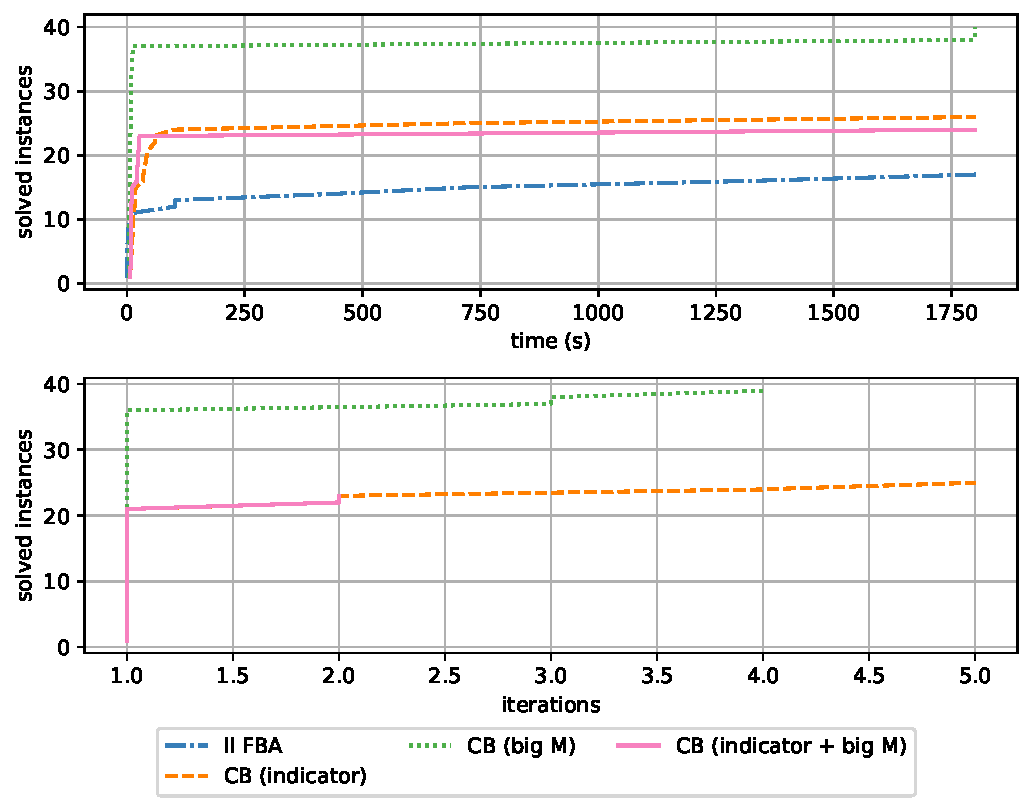
\includegraphics[width=0.8\textwidth]{Images/comparison_solved_instances_gecko_1.0e-8_indicator_and_big_m.pdf}
%     \label{fig:comparison_solved_instances_gecko_1.0e-8_indicator_and_big_m_as_MP}
% \end{figure}


%%%%%%%%%%%%%%%%%%%%%%%%%%%%
%%%%%Ende des Dokuments%%%%%
%%%%%%%%%%%%%%%%%%%%%%%%%%%%
\newpage
\restoreapp